%\documentclass{article}
%\usepackage[utf8]{inputenc}
%\usepackage{graphicx}

%\title{flores}

%\begin{document}

%\section{Caça às flores}

Damiko precisa fazer uma pesquisa sobre $T$ diferentes tipos de flores para a escola.
 Para isso ele irá usar o jardim existente em sua casa para colher esses $T$ tipo de flores.
 Como ele deixou para realizar a pesquisa de última hora, precisa colher as flores de forma rápida e portanto ele necessita de sua ajuda para encontrar a menor área quadrada do jardim que contém todos os tipos de flores (1 a $T$ inclusive).



Sua tarefa é simples.
Damiko irá fornecer um mapa do seu jardim no formato de uma matriz $N \times M$ onde, em cada posição, há um valor inteiro representando os tipos de flores no local.
O $i$-ésimo bit menos significativo desse inteiro é 1 se e somente se nessa posição da matriz existe a flor do tipo $i$. 
% A interpretação desses valores funciona da seguinte forma: O resto da divisão desse número por 2 é um valor binário onde 1 (true) significa que existe a flor do tipo 1 e 0 (false) significa que não existe a flor tipo 1.
% Para a verificação da flor do tipo 2 basta fazer o mesmo procedimento, mas agora para o resultado da divisão da operação anterior.
% Esse ciclo segue até que o resultado da divisão seja 0.
 Portanto se uma posição do jardim contém, por exemplo, o valor 5, isso significa que existem dois tipos de flores: o tipo 1 e o tipo 3.
 Caso o valor seja 7 ela contém os tipos:  1, 2 e 3.
 Caso seja 0, não existem flores no local.

Segue um exemplo de mapa $3 \times 4$ de um jardim com $T=5$ tipos de flores:

\begin{center}
  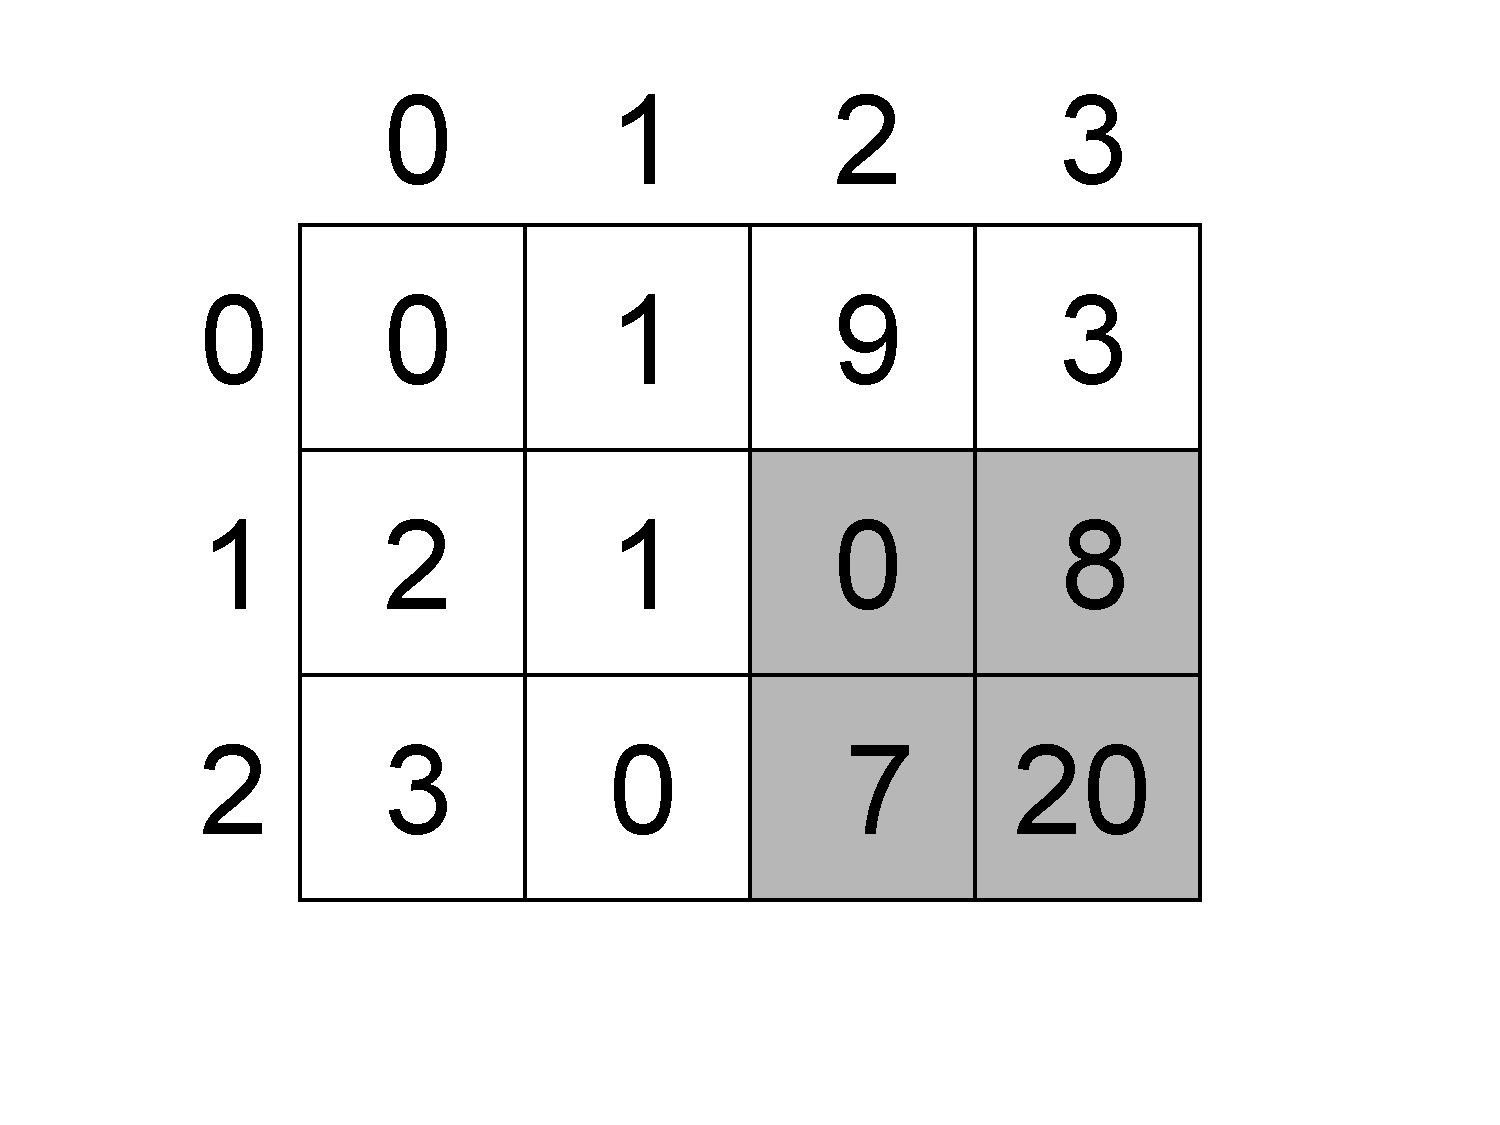
\includegraphics[width=0.4\linewidth]{\CWD/figura.pdf}
\end{center}

No exemplo do jardim acima a menor região que contém os 5 tipos diferentes de flores é a de área 4 destacada iniciando na posição $(1, 2)$ e finalizando na posição $(2, 3)$.


\section*{Entrada}

A primeira linha da entrada contém três inteiros $N$, $M$ e $T$ separados por espaço, onde $N$ e $M$ são as dimensões do jardim e $T$ é o número de tipos flores a serem colhidas. 
Cada uma das $N$ linhas seguintes contém $M$ inteiros separados por espaço. O $j$-ésimo inteiro da $i$-ésima dessas linhas, $X_{ij}$, representa as flores na posição $(i - 1, j - 1)$ do jardim.


\section*{Saída}

Caso seja possível coletar todas as flores colhendo uma área quadrada do jardim, a primeira linha da entrada deve conter um inteiro indicando a menor área quadrada que deve ser coletada. A segunda linha deve conter dois inteiros $L$ e $C$ separados por espaço, indicando respectivamente a linha e a coluna do canto superior esquerdo do quadrado coletado. Caso haja mais de uma resposta possível, escolha uma que minimize $L$. Se, mesmo assim, ainda houver mais de uma resposta possível, escolha aquela que minimiza $C$. Caso não seja possível coletar todas as flores colhendo uma área quadrada do jardim, a saída deve conter uma linha com o inteiro $-1$.

\section*{Restrições}
\begin{itemize}
\item $1 \leq N,M \leq 1000$
\item $1 \leq T \leq 10$
\item $0 \leq X_{ij} \leq 1023$ para todo $i = 0, 1, \ldots, N - 1$, $j = 0, 1, \ldots, M - 1$.
\end{itemize}
\section*{Exemplos}
\exemplo
